% It is advisable to learn the basics of LaTeX before using this template.
% A good resource to start with is http://en.wikibooks.org/wiki/LaTeX/
%
% All template fields are marked with a pair of angular brackets e.g. <title here>
% except for the ones defining citation names in ref.tex.
%
% Empty space after chapter/section/subsection titles can be used to insert text.
%
% Just compile this file using pdflatex after making all required changes.

\documentclass[12pt,a4paper]{report}
\usepackage[pdftex]{graphicx} %for embedding images
\usepackage{url} %for proper url entries
\usepackage{fancyhdr,lipsum}
\pagestyle{fancy}
\renewcommand{\chaptermark}[1]{\markright{\ #1}{}}
\fancyhf{}% Clear header/footer
\fancyhead[L]{\bfseries\rightmark}
\fancyhead[R]{\bfseries\thepage}
\usepackage{listings} %code extracts
\usepackage{xcolor} %custom colours
\usepackage{mdframed} %nice frames
\usepackage{hyperref}
\definecolor{light-gray}{gray}{0.95} %the shade of grey that stack exchange uses

\begin{document}
\renewcommand\bibname{References} %Renames "Bibliography" to "References" on ref page

%include other pages
\begin{titlepage}

\begin{center}

\textup{\large {\bf C207 Final Project} \\ Report/Documentation}\\[0.2in]

% Title
\Large \textbf {Chemical Kinetics Library}\\[0.3in]

       \small \emph{Submitted in fulfillment as per the\\
        requirements of the course}
        \vspace{.2in}

       {\bf CS207 : Systems Development for Computational Science}\\[0.3in]

% Submitted by
\normalsize Submitted by \\
\large \textbf{Group 11} \\
\begin{table}[h]
\centering
\begin{tabular}{lr}\hline \\
Team Members \\ \\ \hline
\\
Karan R. Motwani\\
Hannah Sim\\ 
Shiyu Huang\\
Haixing Yin\\ \\ \hline 
\end{tabular}
\end{table}

\vspace{.1in}
Under the guidance of\\
{\textbf{Prof. David Sondak}}\\[0.2in]

\vfill

% Bottom of the page

\includegraphics[scale=0.65]{logo}\\[0.1in]
\normalsize
\textsc{Harvard University}\\
Cambridge, Massachusetts -- 02138 \\
\vspace{0.3cm}
\textbf{Fall Semester, 2017}
\end{center}

\end{titlepage}

\vspace{2in}
\begin{abstract}
This repository is  collection of Python algorithms and classes intended for research in
Reaction Rate quantification, including the calculation of Reaction Rate Coefficients and Progress Rate for a system of chemical reactions. The library is capable of receiving an XML file as input and extracting the chemical species and quantities of interest for further manipulation. The library is designed for flexibility, extensibility and ease of use. Its software
design follows an object-oriented approach and its code is written on Python over an Anaconda Platform. 
The library consists of three levels of documentation: a model document available in PDF format, comprehensive code documentation within individual Python files and a lower-level user's guide in the README file available in the repository.
This is the model document: it gives a comprehensive overview of the library's capabilities, provides procedures
for software execution, and includes example for ease of use.
\end{abstract} 


\pagenumbering{roman} %numbering before main content starts
\tableofcontents
\listoffigures

\newpage
\pagenumbering{arabic} %reset numbering to normal for the main content

%\chapter{Problem Definition}

<Problem Definition here>
 %objective changed to problem definition
\chapter{Introduction}

\section{Problem Definition}
It is accepted that computation has emerged as the third pillar of science alongside the pillars of theory and experiment. Computational science is maturing rapidly and has found considerable and significant use in supporting scientists from various disciplines. The Chemical Kinetics Library available in this repository aims to ease the process of calculation of Reaction Rate, Reaction Rate Coefficients and Progress Rate of a system of chemical reactions. The tool simplifies the process by orders of magnitude by simply taking a standard XML file as input and returning the desired parameters in suitable data structures. This library has great application in the field of Ordinary Differential Equation (ODE) solving for chemical reactions and can be further extended to more complex applications such as learning new reaction pathways in an artificial neural net based code library. 


\section{Chemical Kinetics : Brief Overview}
In the follow subsections, the essential Chemical Kinetics concepts behind the algorithms and their implementation have been discussed.
\subsection{Reaction Rate and Coefficient}
In chemical kinetics a reaction rate constant or reaction rate coefficient, k, quantifies the rate of a chemical reaction. For a reaction between reactants A and B to form product C :\\
\begin{center}
   $\nu_{A} A + \nu_{B} B \longrightarrow \nu_{C} C.$ 
\end{center}
The reaction rate is often found to have the form :
\begin{center}
   $ r = k(T) [A]^{m} [B]^{n}$ 
\end{center}
Here k(T) is the reaction rate constant that depends on temperature. [A] and [B] are the molar concentrations of substances A and B in moles per unit volume of solution, assuming the reaction is taking place throughout the volume of the solution. (For a reaction taking place at a boundary one would use instead moles of A or B per unit area).\\
\\The exponents \textbf{m} and \textbf{n} are called partial orders of reaction and are not generally equal to the stoichiometric coefficients a and b. Instead they depend on the reaction mechanism and can be determined experimentally.\\
\\The Reaction Rate Coefficient has multiple forms : \\
\begin{center}
   {$&k_{\textrm{const}}   = k \hspace{3.9cm}\tag{\textbf{Constant}}$
\end{center}
\begin{center}
   $&k_{\textrm{arr}}     = A \exp\left(-\frac{E}{RT}\right)$ \hspace{2cm} \tag{\textbf{Arrhenius}}
\end{center}
\begin{center}
   $&k_{\textrm{mod-arr}} = A T^{b} \exp\left(-\frac{E}{RT}\right) \hspace{1cm} \tag{\textbf{Modified Arrhenius}}$
\end{center}
\vspace{0.1in}
The symbols used above are :
\begin{itemize}
    \item The Arrhenius prefactor : $A$
    \item The Modified Arrhenius parameter : $b$
    \item The Temperature : $T$ in Kelvin. 
    \item Activation Energy : $E$ in Joule/mol
    \item $R = 8.314$ is the ideal gas constant (in Joules/ mol K).
\end{itemize}

\subsection{System of Reactions}
Consider a system consisting of $N$ species undergoing $M$ irreversible, elementary reactions of the form :
\begin{center}
     $\sum_{i=1}^{N}{\nu_{ij}^{\prime}\mathcal{S}_{i}} \longrightarrow 
  \sum_{i=1}^{N}{\nu_{ij}^{\prime\prime}\mathcal{S}_{i}}, \qquad j = 1, \ldots, M$
\end{center}
\vspace{0.7in}The Rate of Change of Specie $i$ (the Reaction Rate) can be written as :\begin{center}
     $f_{i} = \sum_{j=1}^{M}{\nu_{ij}\omega_{j}}, \qquad i = 1, \ldots, N$
\end{center}
And the Progress Rate for each reaction is given by :\begin{center}
  $\omega_{j} = k_{j}\prod_{i=1}^{N}{x_{i}^{\nu_{ij}^{\prime}}}, \qquad j = 1, \ldots, M$
\end{center}
and $k_{j}$ is the forward reaction rate coefficient. The symbols used above are :
\begin{itemize}
    \item Chemical symbol of the Specie $i$ : $\mathcal{S}_{i}$
    \item Stoichiometric Coefficients of the Reactants : $\nu_{ij}^{\prime}$
    \item Stoichiometric coefficients of Products : $\nu_{ij}^{\prime\prime}$ 
    \item Rate of consumption or formation of specie $i$ (Reaction Rate) : $f_{i}$ 
    \item Progress Rate of reaction $j$ : $\omega_{j}$
    \item Concentration of Specie $i$ : $x_{i}$
    \item Reaction Rate Coefficient for reaction $j$ : $k_{j}$ 
\end{itemize}
\section{Code Features}
\subsection{Flow of Control}
From the above expressions, it is clear that the terms/parameters of a system of reactions need to be calculated in an specified order. The Reaction and Progress Rate ($\omega_{j}$) depend on the Rate Coefficient ($k_{j}$) and the Concentrations of each Specie (${\nu_{ij}}$) depends on the Reaction Rate ($f_{i}$) and Time ($t$) for which the reaction is allowed to progress. \\
\\The Initial Concentrations of the Reactants ($\nu_{ij}^{\prime}$)  and the Temperature ($T$) need to be input by the user dynamically for a specific reaction to observe the variance of the results for different initial conditions. The Species involved in the system and the type of reaction, however, is pre-defined.\\
\\Abiding by this model, the usage of the library needs to follow an ordered set of operations :
\begin{itemize}
    \item The \textbf{Parser} extracts the Parameters and Species of a chemical reaction from XML file.
    \item In the \textbf{ChemKin} module, the Reaction Rate Coefficient needs to be calculated for an input Temperature and Concentrations using the information about the extracted Parameters.
    \item Finally, the respective Reaction Rate/Progress Rate can be calculated based on Stoichiometric Coefficients, provided as input through the \textbf{Terminal}. 
\end{itemize}

\subsection{Data Structures}
\subsubsection{Classes}
\begin{itemize}
    \item \textbf{class 'ReactionParser'} : The user instantiates an object of this class with the XML filename as an argument, it consists of methods that facilitate the extraction of Type of Reaction, Rate Parameters, Species and Stoichiometric Coefficients from the file.
    \item \textbf{class 'Reaction'} : The class 'ReactionParser' instantiates an object of this class with the parameters obtained from methods of the class 'ReactionParser'. It consists of methods that allow the user definition of Temperature, Concentrations and calculation Progress/Reaction Rate.
    \item \textbf{class 'ReactionCoeff'} : An object of this class is called by method 'compute\_reaction\_rate\_coeff' of class 'Reaction' with the parameters for the calculation of Rate Coefficient in the form of a dictionary and Temperature as arguments. It consists of methods that calculate the Reaction rate Coefficent based on the parameters passed.
\end{itemize}
\subsubsection{Dictionaries}
\begin{itemize}
    \item \textbf{Reaction Rate Parameters} : Parameters such as Activation Energy, Arrhenius pre-factor and Rate Constant are passed as a single dictionary for ease of calculation of Rate Coefficients.
    \item \textbf{Stoichiometric Reactant Coefficients} : The values of the Stoichiometric Reactant Coefficients are stored in a dictionary with the unique species as an index for ease of calculation of Reaction/Progress Rate.
    \item \textbf{Stoichiometric Product Coefficients} : The values of the Stoichiometric Product Coefficients are stored in a dictionary with the unique species as an index for ease of calculation of Reaction/Progress Rate.
\end{itemize}
\subsubsection{Other Data Structures}
\begin{itemize}
    \item \textbf{Lists} : are used to store a collection of the unique species of the system of reactions.
    \item \textbf{Sets} : are used for easy unique-ness check operations at the reaction level.
\end{itemize}
\textbf{} %literature survey included in this
\chapter{Installation}

\section{Downloading the Repository}
The repository is available on \textbf{github} through URL : \url{https://github.com/cs207-group11/cs207-FinalProject.git}. To download :
\begin{itemize}
    \item Below 'Contributors', a green button to 'Clone or download' the repository is present.
    \item Use the 'Download ZIP' option to begin the download.
    \item Once completed, the ZIP file will be present in 'Downloads' folder of your computer (default).
    \item Unzip this file into a directory of your choice using WinRAR or equivalent software.
    \item Now, follow instructions in Chapter 3 : Procedure for usage.
\end{itemize}
This link can also be used to clone the repository to your machine through the Mac Terminal/GitBash.
\begin{itemize}
    \item Enter directory of your choice using appropriate 'cd' commands.
\end{itemize} 
\begin{mdframed}[backgroundcolor=light-gray, roundcorner=10pt,leftmargin=1, rightmargin=5, innerleftmargin=10, innertopmargin=5,innerbottommargin=5, outerlinewidth=1, linecolor=light-gray]
\begin{lstlisting}
$ git clone <repository URL mentioned above>
$ cd cs207-FinalProject
\end{lstlisting}
\end{mdframed} 
You are now in the repository and can follow Chapter 3 : Procedure instructions for usage.
\newpage
\section{Test Suite}
The testing is an important phase of development of any project and a variety of tests are necessary before the design is released. We have defined a test module called 'test\_chemkin.py' within this repository.
\subsection{Types of Errors}
\begin{itemize}
    \item ValueError: check the user's input values for incorrect variable or parameter definitions. Ex : Negative Temperature/Molar Concentration. 
    \item AttributeError: check if the execution of the program is in the right order. Ex : If the Rate Coefficient has been calculated before attempting to calculate the Reaction Rate.
    \item TypeError : checks if the entered parameters are real and belong to a certain data type. Ex : Modified Arrhenius factor 'b' is real and a float.
    \item NotImplementedError : checks if a certain feature/function has been designed or is due for implementation.
\end{itemize}
The above types of errors are tested for within the module 'test\_chemkin.py' for erroneous input to test the robustness of the 'chemkin.py' module.
\subsection{Running the Test Suite}
The test suite can be run from the \textbf{Terminal} to view the results of the testing.
\begin{mdframed}[backgroundcolor=light-gray, roundcorner=10pt,leftmargin=1, rightmargin=5, innerleftmargin=10, innertopmargin=5,innerbottommargin=5, outerlinewidth=1, linecolor=light-gray]
\begin{lstlisting}
#Enter repository directory
>>> python -m pytest test_chemkin.py
\end{lstlisting}
\end{mdframed} 
\chapter{Usage and Examples}
\section{Procedure}
\begin{itemize}
    \item Clone the repository from \textbf{github} onto your local machine.
    \item Copy your target XML file to the directory of the cloned repository and instantiate an object of \textbf{class ReactionParser} with the filename.
    \item The '\_\_call\_\_' method defined for your convenience allows you to begin the extraction of parameters from the XML file.
    \item In addition to the parameters, information about the Stoichiometric Coefficients and Type of Reaction is derived from the XML File for the reactants and products separately.
    \item The object of \textbf{class Reaction} accepts the parameters extracted from the XML file directly through the \textbf{class ReactionParser}.
    \item The Temperature needs to be provided by the user at run-time through a method 'set\_temperature' of the \textbf{class Reaction}.
    \item The Reaction Rate Coefficient is calculated by calling a method 'compute\_reaction\_rate\_coeff' of \textbf{class Reaction} which instantiates an object of \textbf{class ReactionCoeff} and passes a dictionary of parameters necessary for calculation. 
    \item The \textbf{class ReactionCoeff} consists of methods for individual forms of the Reaction Rate Coefficient and returns the coefficient according to the parameters passed as input.
    \item Finally,  the concentrations of the unique species needs to be provided by the user at run-time through a method 'set\_concentrations' of the \textbf{class Reaction}.
    \item Using the Reaction Rate Coefficent, Unique Specie Concentrations and Stochiometric Coefficients, the Reaction Rate and Progress Rate can be obtained using methods 'compute\_reaction\_rate'  and 'compute\_progress\_rate' defined in the \textbf{class Reaction}.
\end{itemize}
\section{Examples}
\subsection{Case 1 : Single Reaction System}
\textbf{Problem :} \\
Calculate the \textbf{Progress Rate} for a reaction of the following form :
\begin{center}
  $\nu_{A} A + \nu_{B} B \longrightarrow \nu_{C} C.$\\
\end{center}
\\Order your concentration vector so that 
\begin{align}
  \mathbf{x} =
  \begin{bmatrix}
    \left$[ [A] [B] [C] ]^{T}$ \\
  \end{bmatrix}
\end{align}
Test your function with 
\begin{align}
  $\nu_{i}^{\prime}$ =
  \begin{bmatrix}
    \left$[2.0 1.0 0.0]^{T}$ \\
  \end{bmatrix}
\end{align}
And concentrations  
\begin{align}
  $x$ =
  \begin{bmatrix}
    \left$[1.0 2.0 3.0]^{T}$ \\
  \end{bmatrix}
\end{align}
Reaction Rate Coefficent : $k = 10$

\begin{flushleft}
\textbf{Solution Code :}
\end{flushleft}

\begin{mdframed}[backgroundcolor=light-gray, roundcorner=10pt,leftmargin=1, rightmargin=5, innerleftmargin=10, innertopmargin=5,innerbottommargin=5, outerlinewidth=1, linecolor=light-gray]
\begin{lstlisting}
#Copy target XML file into repository
>>> parser(xml_filename)
>>> parser()

#Fetch desired reaction index, in this case 0 (zero)
>>> reac1 = parser.reaction_list[0]

#Print Reaction Equation
>>> print(reac1)

#Set Temperature (although not needed for this)
#reac1.set_temperature(1000)
>>> reac1.set_concentrations({'A':1,'C':3,'B':2})

#Order doesn't matter as long as all species exist
>>> k = reac1.compute_reaction_rate_coef()
>>> omega = reac1.compute_progress_rate()

#Reaction Rate can be calculated similarly
>>> print ("Reaction Rate Coefficient =",k)
>>> print ("Progress Rate =",omega)
\end{lstlisting}
\end{mdframed} 
\textbf{Result :}\\
\\
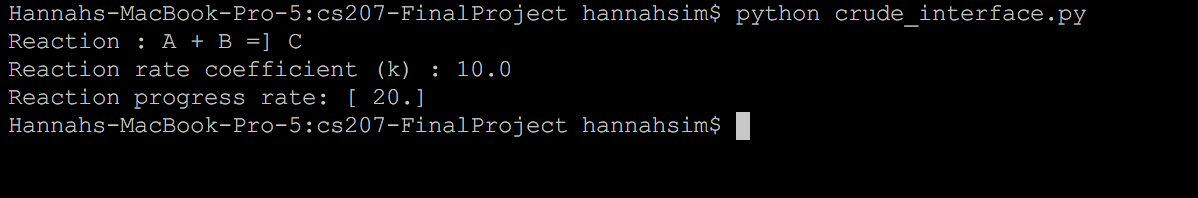
\includegraphics[scale=0.35]{result}
\chapter{Future Work}
In the future, we intend to add a non-trivial feature for simplifying calculations in Chemical Kinetics. 

%\input{conclusion}
%\cleardoublepage
%\pagebreak
\phantomsection
\addcontentsline{toc}{chapter}{Acknowledgements}
\chapter*{Acknowledgments}
\vspace{1.0in}
<Acknowledgements here>
\\
\\
\\ 
\\
<Name here> \\ 
\\
<Month and Year here>\\
{National Institute of Technology Calicut}\\
\newpage
\begin{figure}[htb]
\centering

\includegraphics[scale=0.3]{glider} % e.g. insert ./image for image.png in the working directory, adjust scale as necessary
\caption{<Caption here>}
\label{fig:label} % insert suitable label, this is used to refer to a fig from within the text as shown above
\end{figure}
\cleardoublepage
%\pagebreak
\phantomsection
\addcontentsline{toc}{chapter}{References}
\begin{thebibliography}{99}

\bibitem{citation-1-name-here}Chemical Kinetics : Wikipedia,\ \url{https://en.wikipedia.org/wiki/Chemical_kinetics}
\end{thebibliography}


\end{document}
